% This is samplepaper.tex, a sample chapter demonstrating the
% LLNCS macro package for Springer Computer Science proceedings;
% Version 2.21 of 2022/01/12
%
\documentclass[runningheads]{template/llncs}
%
\usepackage{array}
\usepackage[T1]{fontenc}
% T1 fonts will be used to generate the final print and online PDFs,
% so please use T1 fonts in your manuscript whenever possible.
% Other font encondings may result in incorrect characters.
%
\usepackage{newtxtext,newtxmath}  % BD



\usepackage{graphicx}
\usepackage{amsmath}
\usepackage[utf8]{inputenc}
% Used for displaying a sample figure. If possible, figure files should
% be included in EPS format.
%
% If you use the hyperref package, please uncomment the following two lines
% to display URLs in blue roman font according to Springer's eBook style:
% \usepackage{color}
% \renewcommand\UrlFont{\color{blue}\rmfamily}
% \urlstyle{rm}
%

% BD:
\usepackage{booktabs}
\usepackage{enumitem}
\usepackage{pgfgantt}

% \numberwithin{figure}{section}
% \numberwithin{table}{section}

\newcommand{\m}[2]{$M^{#1,#2}$}

\begin{document}
%
\begin{titlepage}
    \begin{center}
        
        
\includegraphics[width=0.6\textwidth]{template/VU_logo.pdf}
        \vspace{0.8cm}
        
        \large \text{Project Proposal}
        \vspace{0.2cm}
        
        \noindent\rule{\linewidth}{1pt}
        {\fontsize{15pt}{20pt}\selectfont\textbf{Thesis Title: Concise and Engaging Title}}
        \noindent\rule{\linewidth}{1pt}
        \vspace{0.1cm}
        
        \text{by}\\
        \vspace{0.5cm}
        \textbf{Bas Diender} \\ 
        {(2711178)}
        \vspace{2cm}

        
        {\fontsize{12pt}{14pt}\selectfont
        \begin{tabular}{>{\raggedleft}p{4cm} @{\hspace{1pt}: \hspace{2pt}} l}
        \textit{First Supervisor} & Name and Surname \\
        \textit{Daily Supervisor} & Name and Surname \\
        \textit{Second Reader} & Name and Surname \\
        \end{tabular}
        }
       
        \vspace{3cm}
        
        % {\large June 4, 2025}
        \vfill
        
        % {\fontsize{13pt}{14pt}\selectfont
        % Submitted in partial fulfillment of the requirements for\\ the VU degree of Master of Science in Artificial Intelligence}
    \end{center}
\end{titlepage}

\title{Project Proposal}
%
%\titlerunning{Abbreviated paper title}
% If the paper title is too long for the running head, you can set
% an abbreviated paper title here
%
\author{Bas Diender}
%
\authorrunning{B. Diender}
% First names are abbreviated in the running head.
% If there are more than two authors, 'et al.' is used.
%
\institute{Vrije Universiteit Amsterdam, Amsterdam, The Netherlands}
%
\maketitle
% Start with a brief introduction into the problem that your research will address, or the novel insights it is intended to yield, convincing the reader of the societal and scientific relevance of the task. If you do an external internship, also give the context of the internship provider. The intro may end with one or more research questions and/or a problem statement.

\section{Introduction}
\label{sec:introduction}
	Language models like BERT~\cite{devlin-etal-2019-bert} have become a cornerstone technology in NLP research. In short, they are trained for next-word prediction in large datasets of text and, in doing so, pick up on linguistic properties that can be leveraged in a wide variety of downstream language-related tasks. Multilingual language models (MLMs) are trained on texts in many different languages. In the process, they pick up on both linguistic properties that are shared across all languages, as well as language-specific properties shared by only a subset of all languages. As a consequence, an MLM can bootstrap knowledge obtained from one language when dealing with another language in a process called \textbf{cross-lingual transfer}. This is particularly advantageous for low-resource languages. Such languages may not have enough data for a language model to adequately pick up on the language's patterns; however, in a multilingual setting, the model can use the patterns it picks up from more well-resourced languages in its training data.

	Some linguistic patterns are language-universal, such as the presence of a subject-predicate structure to express who is doing what; whereas others are present only in a subset of the world's languages, such as strictly positioning a subject in front of its predicate. The study of which languages exhibit which patterns is called \textbf{linguistic typology}.~\cite{croft-2002-typology} It is intuitive that an MLM's ability to leverage properties of one language to improve its understanding of another depends on the typological similarity between the two languages. Given the importance of cross-lingual transfer for improving performance on low-resource languages, it is important to subject this intuition to scrutiny. Hence, the goal of this project is to investigate the role of typology in an MLM's adaptability to other languages. In particular, it aims to assess the following hypotheses:

	\begin{list}{}{\leftmargin=1em \rightmargin=1em}
		\item
		\begin{enumerate}[label=\textbf{H\arabic*:}, leftmargin=*, align=left]
		    \item When adapting to a typologically similar language, changes to the model parameters are less extensive than when the model adapts to a more distant language;
		    \item When adapting to a typologically similar language, changes to the model parameters are minimal in the layers responsible for handling syntactic features;
		    \item The performance of an MLM in a few-shot setting is positively correlated with the typological similarity to the languages it has already adapted to.
		\end{enumerate}
	\end{list}


	\noindent The corresponding research questions are as follows:

	\begin{list}{}{\leftmargin=1em \rightmargin=1em}
		\item
		\begin{enumerate}[label=\textbf{Q\arabic*:}, leftmargin=*, align=left]
			\item How is typological distance reflected in the model parameters? (H1, H2)
			\item How does typological distance affect cross-lingual transfer, as reflected by downstream performance? (H3)
		\end{enumerate}
	\end{list}

% Discuss the scientific literature that addresses the same or a similar problem as your study, and make clear how your study relates and adds to this body of research. Try to give a broad but concise overview of the ways in which the problem is approached in other studies. 

\section{Related Work}

The link between typological similarity and successful cross-lingual transfer is well established. Pires et al.~\cite{pires-etal-2019-multilingual} found that typological similarity correlates positively with zero-shot learning performance. While they attributed their results to lexical overlap between the source and target languages, Karthikeyan et al.~\cite{karthikeyan-etal-2020-cross} found the same results when the source and target languages had no lexical overlap at all. Instead, they demonstrated structural similarity between two languages to be of greater importance.

Typological relatedness has informed cross-lingual research in low-resource settings, too. Nooralahzadeh et al.~\cite{nooralahzadeh-etal-2020-zero} use a multi-stage approach to cross-lingual transfer with MAML where between the initial stage of fine-tuning on a large dataset to instill task-specific knowledge and few-shot learning to low-resource languages, they fine-tune on auxiliary languages to optimize the model parameters for quick adaptation. Choenni et al.~\cite{choenni-etal-2023-cross} adapt this method and match auxiliary languages and low-resource languages based on typological similarity to further facilitate cross-lingual transfer.

Tenney et al.~\cite{tenney-etal-2019-bert} set out to quantify where specific types of linguistic information are encoded in BERT, and found each consecutive layer to handle incrementally high-level linguistic information. That is, earlier layers handle concrete features like parts-of-speech tagging, whereas more abstract information like dependency relations and coreference resolution is dealt with in later layers. In the multilingual setting, Choenni \& Shutova~\cite{choenni-shutova-2022-investigating} found that M-BERT's internal representations have a clear typological organization, with the model encoding typological features explicitly and jointly across languages.

This joint encoding could be what underlies the relation between typological similarity and successful cross-lingual transfer. Fine-tuning an MLM on any given language could see it increase the importance of the encodings of the typological features of that language. As a result, after fine-tuning, the model's parameters would be close to what they would have been if the model had been fine-tuned to a typologically similar language.

% % Specify and motivate the proposed approach(es) that you will implement / apply. If it includes a pipeline or architecture, it makes sense to give a rough visualization and description.

\section{Methodology}
\label{sec:methodology}

The methodology follows Choenni et al.~\cite{choenni-etal-2023-cross} in adapting a three-stage fine-tuning setup outlined in Section~\ref{sub:training_setup}, with the model being fine-tuned for dependency parsing in a variety of languages. The choice for dependency parsing was based on the availability of uniform datasets in a wide variety of languages through Universal Dependencies (UD)~\cite{nivre-etal-2016-universal}. The selection of languages is clarified in Section~\ref{sub:languages}, the specifics of the model are discussed in Section~\ref{sub:model}.

\subsection{Model}
\label{sub:model}
	Following Choenni et al.,~\cite{choenni-etal-2023-cross} the model used is derived from UDify,~\cite{kondratyuk-straka-2019-75} which is itself based on M-BERT~\cite{devlin-etal-2019-bert}. UDify incorporates a layer attention mechanism that scales each layer for its importance to the task at hand. That is, during fine-tuning, a weighted sum $\mathbf{e}_j$ is computed for input token $j$ over all layers $i \in [1, ..., 12]$ as follows:

	$$
		\mathbf{e}_j = \sum_i\mathbf{U}_{i,j} \cdot \text{softmax}(\mathbf{w})_i
	$$

	\noindent where $\mathbf{U}_{i,j}$ is the output of layer $i$ at token position $j$ and $\mathbf{w}$ is a vector trained alongside the model such that $\mathbf{w}_i$ reflects the importance of layer $i$. Dependency arcs between tokens are scored using a biaffine attention classifier,~\cite{dozat-manning-2016-deep} after which the optimal parse tree is decoded using the Chu-Liu/Egmonds algorithm.~\cite{chu-1965-shortest}


\subsection{Fine-tuning setup}
\label{sub:training_setup}
	As stated, the fine-tuning setup follows three stages adapted from Choenni et al.~\cite{choenni-etal-2023-cross}

	In the first stage, the model $M$ is fine-tuned on a German-language (\textit{deu}) treebank to instill general knowledge of the task at hand. In the second stage, four copies of $M$ are fine-tuned separately on treebanks of auxiliary languages $\ell \in \{\textit{nld}\textit{swe}\textit{ces}, \textit{hun}\}$\footnote{Dutch, Swedish, Czech, and Hungarian.} to obtain four instances of $M^\ell$. Finally, each $M^\ell$ is fine-tuned on each low-resource language $\lambda \in \{\textit{gsw}, \textit{fao}, \textit{hsb}, \textit{vep}\}$,\footnote{Swiss German, Faroese, Upper Sorbian, and Veps.} resulting in 16 instances of \m{\ell}{\lambda}. If time permits, both the second and third stage are ideally repeated across at least five random seeds.

% \subsection{Languages}
% \label{sub:languages}

% The selection of languages is based on their prevalence in the pre-training data for mBERT and their typological relatedness. For typological relatedness, the syntactic feature-vectors (\texttt{syntax\_knn}) from the URIEL knowledge base~\cite{littell-etal-2017-uriel} are used. Languages are then presented as vectors encoding their typological features, and relatedness is taken to be the cosine similarity between those vectors.

% The initial language German is chosen as one of the most well-represented languages in mBERT's pre-training data.~\cite{wu-dredze-2020-languages} Moreover,~\cite{turc-etal-2021-revisiting} found German (alongside Russian) to be the most effective language for cross-lingual transfer. The intermediary languages are then selected as they have roughly the same amount of pre-training data for mBERT. In addition, they each represent a different level of relatedness to German: Phylogenetically, Hungarian and German are entirely unrelated; Czech and German are both part of the Indo-European language family, but are respectively part of the Slavic and Germanic branches; Swedish and German are both Germanic languages, but are respectively part of the North and West Germanic subbranches; and Dutch and German are both members of the West Germanic subbranch. As shown in Figure~\ref{fig:hcd}, this phylogenetic structure is also captured by a hierarchical clustering analysis of the languages' \texttt{syntax\_knn} vectors.


\subsection{Languages}
\label{sub:languages}
	Broadly speaking, language selection is based on their typological similarity and their prevalence in M-BERT's pre-training data as reported by Wu \& Dredze.~\cite{wu-dredze-2020-languages} Typological similarity is defined using the syntactic feature-vectors (\texttt{syntax\_knn}) from the URIEL knowledge base.~\cite{littell-etal-2017-uriel} In particular, each language is represented as a feature-vector, and similarity between languages is taken to be the cosine similarity between their respective vectors.

	German was selected as one of the most prominent languages in M-BERT's pre-training data. Moreover, Turc et al.~\cite{turc-etal-2021-revisiting} found German (alongside Russian) to be the most effective language for cross-lingual transfer. The auxiliary languages all have a roughly similar amount of data in M-BERT's pre-training data. Their selection is motivated phylogenetically, as they each represent a different level of relatedness to German (Hungarian is unrelated, Czech is in the same family, Swedish is in the same branch, Dutch is in the same subbranch). However, a hierarchical clustering analysis of the \texttt{syntax\_knn} vectors (Appendix~\ref{app:a}) found their selection to by typologically valid, too.


% For the final set of languages, the most similar languages from a selection of low-resource languages included in UD were found for each of the intermediary languages. For Dutch and Swedish, these were found to be Swiss German and Faroese, respectively. However, the similarity between those pairs was found to be considerably higher than the similarity between Czech, Hungarian, and their respective most similar languages\,---\,Upper Sorbian and Veps. Since the cosine similarity between Dutch and Faroese was found to be more comparable, the decision was made to disregard Swedish in the final stage and to match Dutch with Faroese.

% % \begin{table}
% % \centering
% % \label{tab:selection}
% % 	\begin{tabular}{lll}
% % 		\toprule
% % 		\textbf{Language} & \textbf{WikiSize} & \textbf{Family}\\
% % 		\midrule
% % 		  German & 12 & IE, Germanic, West\\
% % 		  \addlinespace
% % 		  Dutch & 10 & IE, Germanic, West\\
% % 		  Swedish & 10 & IE, Germanic, North\\
% % 		  Czech & 10 & IE, Slavic, West\\
% % 		  Hungarian & 10 & Uralic, Ugric\\
% % 		  \addlinespace
% % 		  Faroese & --- & IE, Germanic, North\\
% % 		  Upper Sorbian & --- & IE, Slavic, West\\
% % 		  Veps & --- & Uralic, Finnic\\
% % 		\bottomrule
% % 	\end{tabular}
% % 	\caption{Languages used for experimentation. WikiSize is $\log_2$ of the size (in MB) of the portion of mBERT's pre-training data for that specific language, rounded to the nearest integer, as reported by~\cite{wu-dredze-2020-languages}.}
% % \end{table}

% % Describe what the experiment(s) will look like. Depending on your study, it can include information like:
% %%% Research design
% %%% Dataset (including information on source, size, labelling, etc., to the extent available)
% %%% The different variations of the approach that you will compare, as well as details on how they will be applied (library, parameter tuning, etc.) 
% %%% Participants (numbers, intended characteristics)
% %%% Experimental procedure
% %%% Evaluation procedure / metrics

\section{Experimental Setup}
The goal of the project is twofold: Firstly, it aims to show how typology relates to model parameter updates in the fine-tuning stage; secondly, it aims to investigate the effect of typological distance on the success of cross-lingual transfer. Section~\ref{sub:analyses} shows how the setup outlined in Section~\ref{sub:training_setup} serves to achieve these goals. Section~\ref{sub:parameters} lists the parameters used, Table~\ref{tab:data} in Appendix~\ref{app:b} lists the specific datasets used in the experiments.

	\subsection{Analyses}
	\label{sub:analyses}
		\subsubsection{Q1}
		In the second stage, four model instances optimized for dependency parsing in German is fine-tuned to do dependency parsing in languages with varying levels of similarity to German. Intuitively, the German-language data in the preceding stage would have prepared it for dependency parsing in the closely related Dutch more than in the unrelated Hungarian. H1 would suggest that the model instance that fine-tunes to Dutch sees less extensive parameter udpates than the one that fine-tunes to Hungarian. In addition, H2 suggests that the updates should primarily be to the earlier layers of the model for Dutch, whereas for Hungarian, they would be across all layers.

		The fine-tuning setup includes learned scalar weights $\mathbf{w}_i$ that indicate the importance of each layer $i$. Following Tenney et al.~\cite{tenney-etal-2019-bert}, these can be used to detect where model updates took place for each $\ell$. With $\Delta\mathbf{w}^\ell = \mathbf{w}^\ell - \mathbf{w}^{\textit{deu}}$ being the shift in layer importance after fine-tuning on $\ell$, the expectation is that $\Delta\mathbf{w}^{\textit{nld}}_i$ is greater for layers $i$ that deal with lexical information (i.e., the earlier ones~\cite{tenney-etal-2019-bert}), but lower for layers $i$ that deal with higher-level typological features, since those are generally shared between Dutch and German. On the other hand, the values of $\Delta\mathbf{w}^{\textit{hun}}$ are expected to be more uniform, since Hungarian differs significantly from German both lexically and syntactically.

		\subsubsection{Q2}
		In the third stage, the model instances for languages $\ell$ are fine-tuned further to each the low-resource languages $\lambda$. Each \m{\ell}{\lambda} is then evaluated on the test set for $\lambda$, with performance measured as the Labeled Attachment Score (LAS). H3 suggests that greater cosine similarity $s(\ell, \lambda)$ should correspond to higher performance on $\lambda$'s test set.

	\subsection{Parameters}
	\label{sub:parameters}
		The model is first fine-tuned to Part A\footnote{The HDT treebank training data is split into various parts. With Part A being larger than the entire English-language treebank used by Choenni et al.~\cite{choenni-etal-2023-cross}, the decision was made to use just that part for training.} of the German training set. Choenni et al.~\cite{choenni-etal-2023-cross} use the English EWT treebank with \~12.5k samples in this stage and train for 60 epochs. To match the number of examples in this setup, training on the German treebank spans 11 epochs. In the second stage, the model instances are fine-tuned over 1\,000 iterations with a batch size of 20 for all languages $\ell$. In the third stage, the models are fine-tuned on 20 examples sampled randomly from each treebank of language $\lambda$. For the Upper Sorbian treebank, these are sampled from the train set. The other three treebanks do not split their data into separate sets; therefore, the sampled examples are removed from the dataset so as to prevent evaluating on them. 

		Following Choenni et al.~\cite{choenni-etal-2023-cross}, a cosine-based learning rate scheduler with 10\,\% warm-up and the Adam optimizer are used. For the language model, a learning rate of $1e-04$ is used, and for the classifier, a learning rate of $1e-03$ is used.

% Specify the different stages of your research, and their intended duration. You are free to choose how you want to display the planning. A gantt chart is a popular way to do so, as it can represent overlap between stages. Make sure to book in writing throughout the trajectory, and it is advisable to count back from the intended end date of your thesis to know when you would like to finalize your concept version and when the experimentation should be finished to make this happen.

\section{Planning}


\rotatebox{90}{
	\begin{ganttchart}[
	    hgrid,
	    vgrid,
	    x unit=0.2cm,
	    time slot format=isodate-yearmonth,
	    milestone/.append style={fill=yellow!70!brown},
	    bar/.append style={fill=cyan!60!blue},
	    group/.append style={fill=gray!30}
	  ]{2025-04-14}{2025-07-04}

	  \gantttitlecalendar{month=shortname} \\

	  % UDify setup group
	  \ganttgroup{Coding + Experiments}{2025-04-14}{2025-06-04} \\
	  \ganttbar{Understand existing code}{2025-04-14}{2025-04-17} \\
	  \ganttbar{Adapt code}{2025-04-22}{2025-04-30} \\
	  \ganttbar{Set up SLURM scripts}{2025-05-01}{2025-05-02} \\
	  \ganttbar{Run experiments}{2025-05-02}{2025-06-04} \\

	  % Writing tasks
	  \ganttgroup{Writing}{2025-05-06}{2025-07-04} \\
	  \ganttbar[bar/.append style={fill=orange!60!brown}]{Background}{2025-05-06}{2025-05-16} \\
	  \ganttbar[bar/.append style={fill=orange!60!brown}]{Methodology}{2025-05-19}{2025-05-23} \\
	  \ganttbar[bar/.append style={fill=orange!60!brown}]{Results + Discussion}{2025-05-26}{2025-06-04} \\
	  \ganttbar[bar/.append style={fill=orange!60!brown}]{Introduction + Conclusion}{2025-06-05}{2025-06-13}\\
	  \ganttbar[bar/.append style={fill=orange!60!brown}]{Incorporate feedback}{2025-06-23}{2025-07-04}\\

	  \ganttbar[bar/.append style={fill=yellow!70!brown}]{Buffer}{2025-06-16}{2025-06-20}

	\end{ganttchart}
}


\bibliographystyle{plain}
\bibliography{bibliography/anthology}

\newpage

\appendix
\section{Appendix}
\label{app:a}
\begin{figure}
	\centering
	\label{fig:hcd}
		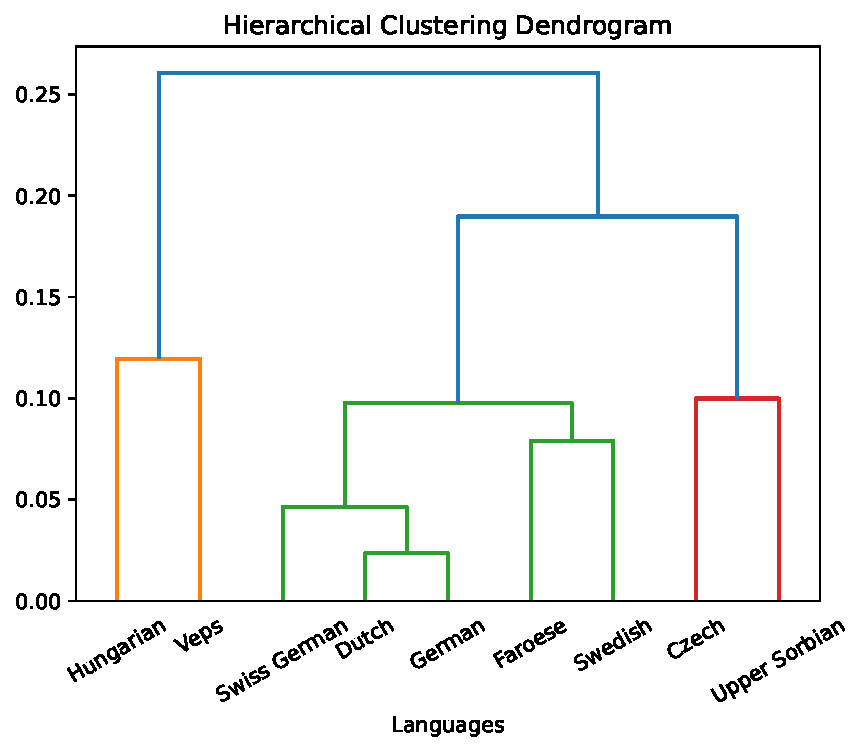
\includegraphics[width=0.60\linewidth]{figures/hcd.pdf}
		\caption{Agglomerative Hierarchical Clustering dendrogram based on the cosine similarity of the \texttt{syntax\_knn} vectors of the included languages.}
\end{figure}

\section{Appendix}
\label{app:b}

\begin{table}
\centering
\label{tab:data}
	\begin{tabular}{llrr}
		\toprule
		\textbf{Language} & \textbf{Treebank} & \multicolumn{1}{l}{\textbf{Number of tokens}} & \multicolumn{1}{l}{\textbf{Number of sentences}} \\
		\midrule
			Czech & CAC & 494\,142 & 24\,709 \\
			Dutch & LassySmall & 297\,486 & 17\,120 \\
			Faroese & OFT & 10\,002 & 1\,208 \\
			German & HDT & 3\,399\,390 & 189\,928 \\
			Hungarian & Szeged & 42\,032 & 1\,800 \\
			Swedish & Talbanken & 96\,859 & 6\,026\\
			Swiss German & ATB & 652 & 98\\
			Upper Sorbian & UFAL & 11\,196 & 646 \\
			Veps & VWT & 1\,303 & 103 \\
		\bottomrule
	\end{tabular}
	\caption{The specific UD treebanks featured in the project.}
\end{table}
\end{document}
